\documentclass[]{tukediphc}
%% -----------------------------------------------------------------
%% tento subor ma kodovanie utf-8
%%
%% na kompilaciu pouzivajte format pdfcslatex 
%%
%% vytvorene distribuciou texlive 2009-7, OS GNU/Linux
%% vytvorene distribuciou TeXLive 2010, OS Win XP
%% februar 2013
%% -----------------------------------------------------------------
\usepackage[utf8]{inputenc}
%\usepackage[T1]{fontenc}
\usepackage{lmodern,textcase}
\usepackage[slovak]{babel}\renewcommand{\figurename}{Obr\'azok}
\def\refname{Zoznam pou\v{z}itej literat\'ury}
\usepackage{latexsym}
\usepackage{dcolumn} % zarovnanie cisiel v tabulke podla des. ciarky
\usepackage{hhline}
\usepackage{subfig}
\usepackage{amsmath}
\usepackage{nicefrac} % pekne zlomky
\usepackage{upgreek} % napr. $\upmu\mathrm{m}$ pre mikrometer ...
\usepackage[final]{showkeys}%color%notref%notcite%final
\usepackage[slovak,noprefix]{nomencl}
\makeglossary % prikaz na vytvorenie suboru .glo
\usepackage{parskip}% 'zhusti' polozky obsahu
%%
%\usepackage[dvips]{graphicx}
%\DeclareGraphicsExtensions{.eps}
\usepackage[pdftex]{graphicx}
\DeclareGraphicsExtensions{.pdf,.png,.jpg,.mps}
\graphicspath{{figures/}} % priecinok na obrazky
%%
%% Cislovane citovanie
%\usepackage[numbers]{natbib}
%%
%% Citovanie podľa mena autora a roku
\usepackage{natbib} \citestyle{chicago}
% -----------------------------------------------------------------
%% tlač !!!
\usepackage[pdftex,unicode=true,bookmarksnumbered=true,
bookmarksopen=true,pdfmenubar=true,pdfview=Fit,linktocpage=true,
pageanchor=true,bookmarkstype=toc,pdfpagemode=UseOutlines,
pdfstartpage=1]{hyperref}
\hypersetup{%
baseurl={http://www.tuke.sk/sevcovic},
pdfcreator={pdfcsLaTeX},
pdfkeywords={Riadenie procesov, Oceliarstvo, Vizualizácia, Virtuálna realita, Matematické modelovanie},
pdftitle={Písomná príprava k predmetu Matematické metódy identifikácie, modelovania a simulácie},
pdfauthor={Michal Takáč},
pdfsubject={Dizertačná skúška}
} 
%% nehodiace zakomentujte !
%\dippraca{Písomná príprava k predmetu Riadenie procesov}
%\bakpraca{Príprava na dizertačnú skúšku}
%%
\nazov{Písomná príprava k predmetu Matematické metódy identifikácie, modelovania a simulácie}
%% ked praca nema 'podnazov' zakomentujte nasledujuci riadok
%% alebo polozku nechajte prazdnu
\podnazov{}
\autor{Ing.~Michal Takáč}
\veduciprace{prof.~RNDr.~Igor~Podlubný, DrSc.}
\univerzita{Technická univerzita v~Košiciach}
\fakulta{Fakulta baníctva, ekológie, riadenia a geotechnológií}
\skratkafakulty{FBERG}
\katedra{Ústav riadenia a informatizácie výrobných procesov}
\skratkakatedry{URIVP}
\odbor{Riadenie procesov}
\specializacia{Kybernetika}
\abstrakt{Abstrakt je povinnou súčasťou každej práce. Je výstižnou
charakteristikou obsahu dokumentu. Nevyjadruje hodnotiace stanovisko
autora. Má byť\/ taký informatívny, ako to povoľuje podstata práce.
Text abstraktu sa píše ako jeden odstavec. Abstrakt neobsahuje odkazy
na samotný text práce. Mal by mať\/ rozsah 250 až 500 slov. Pri
štylizácii sa používajú celé vety, slovesá v činnom rode a tretej
osobe. Používa sa odborná terminológia, menej zvyčajné termíny,
skratky a~symboly sa pri prvom výskyte v texte definujú.}
\klucoveslova{Riadenie procesov, Oceliarstvo, Vizualizácia, Virtuálna realita, Matematické modelovanie}
\datumodovzdania{30. 5. 2020}
\mesto{Košice}

\begin{document}
\renewcommand\theHfigure{\theHsection.\arabic{figure}}
\renewcommand\theHtable{\theHsection.\arabic{table}}
\bibliographystyle{dcu}

\prvastrana


\thispagestyle{empty}
\tableofcontents
\newpage
%
%\thispagestyle{empty}
%%\addcontentsline{toc}{section}{\numberline{}Zoznam obrázkov}
%\listoffigures
%\newpage
%
%\thispagestyle{empty}
%%\addcontentsline{toc}{section}{\numberline{}Zoznam tabuliek}
%\listoftables
%\newpage

%%%%%%%%%%%%%%%%%%%%%%%%%%%%%%%%%

\setcounter{page}{1}
\setcounter{equation}{0}
\setcounter{figure}{0}
\setcounter{table}{0}

\section{Úvod}

%The objective of process control is to keep key process-operating parameters within narrow bounds of the reference value or setpoint. Controllers are used to automate a human function in an effort to control a variable. A basic controller can keep an individual loop on an even point, so long as there is not too much disruption. Complex processes like ones in metallurgy might employ dozens or even hundreds of such controllers, but keeping an~eye on the big picture was, until not so long ago, a human process \cite{Al-Megren2016}.
%
%Cieľom riadenia procesu je udržiavať kľúčové parametre prevádzky procesu v úzkom rozmedzí referenčnej hodnoty alebo požadovanej hodnoty. Ovládače sa používajú na automatizáciu ľudskej funkcie v snahe ovládať premennú. Základný ovládač môže udržiavať jednotlivú slučku na rovnomernom mieste, pokiaľ nedôjde k prílišnému prerušeniu. Komplexné procesy, ako sú procesy v metalurgii, môžu zamestnávať desiatky alebo dokonca stovky takýchto regulátorov, ale pozor na celkový obraz bol až donedávna ľudským procesom \cite{Al-Megren2016}
%
%Although a device was used to automate a human function in an effort to control a variable, there was no sense of what the process was doing overall. A basic controller could keep an individual loop on an even keel, more or less, so long as there was not too much disruption. Complex processes might employ dozens or even hundreds of such controllers, each with its performance displayed on a panel board, but keeping an eye on the big picture was still a human process.	
%
%Aj keď sa zariadenie používalo na automatizáciu ľudskej funkcie v snahe ovládať premennú, nemal zmysel, čo tento proces celkovo robí. Základný ovládač by mohol udržiavať individuálnu slučku na rovnomernom kýli viac alebo menej, pokiaľ nenastane príliš veľa prerušenia. Komplexné procesy môžu využívať desiatky alebo dokonca stovky takýchto kontrolérov, z ktorých každý má svoj výkon zobrazený na doske, ale pozor na celkový obraz bol stále ľudský proces.
%
%The need for developing improved control systems has traditionally been powered by the demand for more accurate and cost efficient production. This is still a major driving force but environmental issues do also have a profound influence on this development today (\cite{Widlund1998}).
%
%Potreba vývoja zdokonalených systémov riadenia bola tradične poháňaná požiadavkou presnejšej a nákladovo efektívnejšej výroby. Je to stále hlavná hnacia sila, ale environmentálne otázky majú na tento vývoj zásadný vplyv aj dnes (\cite{Widlund1998}).
%

%The fast dynamics of the LD converter steelmaking process or the BOF process, as it is commonly known, often makes it a challenge to obtain stable blowing conditions and to achieve the required steel composition and temperature simultaneously at the end point. For this reason, process control becomes very necessary and attempts had started as early as in the 1970s (\cite{Fritz2005}). Out of the originally very simple LD process have grown the modern process-controlled and automated production systems that enable present-day adaptations to meet today’s economic and ecological demands (\cite{Sarkar2015}). The non-linear nature of chemical and thermodynamical processes in basic oxygen steelmaking also amassed interest in developing new mathematical models based on fractionalorder calculus.

Matematický model predstavuje súbor funkčných vzťahov, ktoré transformujú vstupné hodnoty na výsledky, ktorými je možné vyjadriť podstatu modelovaného deja. Modelovanie je pravdepodobne najdôležitejšia časť procesu simulácie. Jej cieľom je čo najpresnejšie zachytiť správanie sa reálneho systému. Zahŕňa identifikáciu problému a očakávaný cieľ riešenia problému, zber reálnych dát alebo generácia náhodných dát, vytvorenie modelu, jeho úprava, prispôsobovanie a jeho overenie porovnaním výstupných dát zo simulácie s reálnymi dátami z reálneho systému.

Procesy výroby ocele všeobecne zahŕňajú základnú kyslíkovú pec, elektrickú oblúkovú pec alebo ekvivalentnú, panvu a kontinuálne liatie a obsahujúce medzipanvu a plesne. Všetky tieto kroky spracovania ocele zahŕňajú vysoko spojené komplexné dopravné javy.

Hlavným cieľom riadenia výroby ocele s kyslíkovým konvertorom je získanie predpísaných parametrov pre oceľ, keď sa odoberá z pece, vrátane hmotnosti, teploty a obsahu každého prvku. V praktickom procese výroby ocele sa o konečnom obsahu uhlíka a teplote často rozhoduje o tom, či je roztavená oceľ prijateľná alebo nie \cite{Wang2010}.


\section{Matematické metódy}

Parciálne diferenciálne rovnice popisujú fyzikálne procesy pohybu tekutín.

Po špecifikovaní problému, ktorý chceme riešiť, je nutné zostaviť sústavu rovníc popisujúcich problém a zvoliť počiatočné, respektíve okrajové podmienky. Je všeobecne známe, že fyzikálne javy v oblasti dynamiky tekutín

%\begin{figure}[ht!]
%	\centering
%	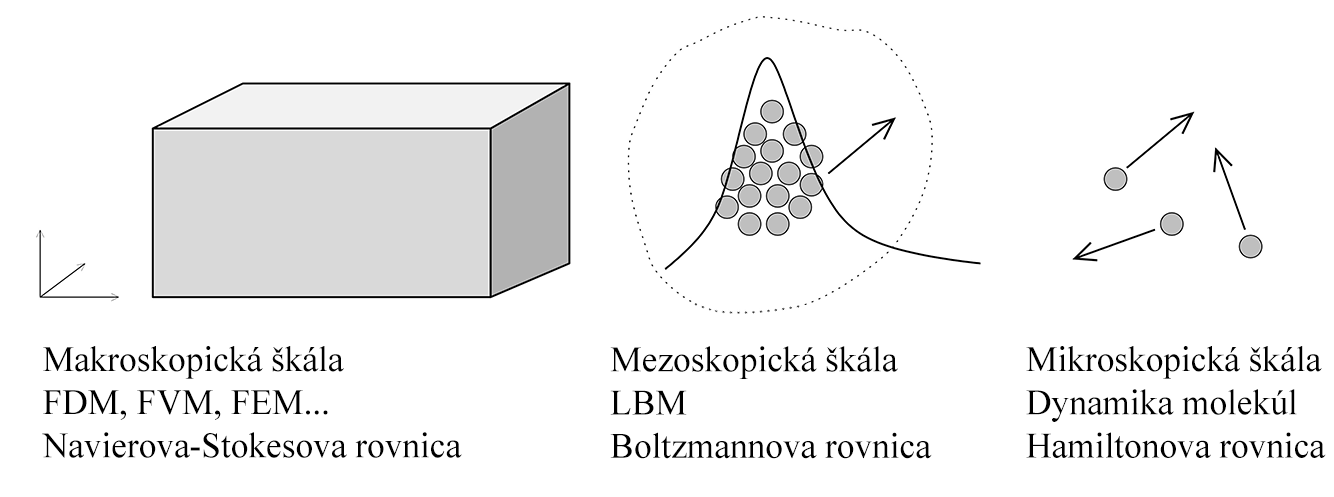
\includegraphics[width=.35\textwidth,angle=0]{figures/different-scales.png}
%	\caption{Rôzne škály.}
%	\label{o:30}
%\end{figure}

\section{Počítačom podporované matematické modelovanie}

Počítačom podporované inžinierstvo (CAE - Computer Aided Engineering) je použitie počítačového softvéru na simuláciu výkonu s cieľom vylepšiť návrhy výrobkov alebo pomôcť pri riešení technických problémov pre celý rad priemyselných odvetví. To zahŕňa simuláciu, validáciu a optimalizáciu produktov, procesov a výrobných nástrojov.

Typický proces CAE pozostáva z krokov predbežného spracovania, riešenia a následného spracovania. Vo fáze predspracovania inžinieri modelujú geometriu (alebo reprezentáciu systému) a fyzikálne vlastnosti návrhu, ako aj prostredie vo forme aplikovaného zaťaženia alebo obmedzení. Ďalej je model vyriešený pomocou vhodnej matematickej formulácie základnej fyziky. Vo fáze po spracovaní sa výsledky predložia technikovi na preskúmanie.

Aplikácie CAE, výhody používania CAE...

\url{https://www.plm.automation.siemens.com/global/en/our-story/glossary/computer-aided-engineering-cae/13112}

Motivácia na používanie počítačových simulácií na skúmanie metalurgických procesov je dvojaká. Po prvé, umožňuje testovať zmeny dizajnu pred vytvorením prototypu, čo samozrejme vedie k nižším celkovým nákladom na návrh. Po druhé, umožňuje skúmať javy, ktoré sa nedajú ľahko merať alebo pozorovať v procese. Dokonca aj zdanlivo jednoduchá operácia, ako napríklad nepretržité meranie teploty počas procesu oduhličovania, je zložitá z dôvodu veľmi vysokých teplôt v procese a všeobecne drsných podmienok prevládajúcich v oceliarňach \citep{Ersson2018}.




V metalurgii pri výrobe ocele je veľmi dôležité simulovať lineárne a nelineárne procesy, s ktorými sa pri výrobe ocele stretávame pri tvorbe matematických modelov. Od prvých pokusov o využitie matematických techník na simuláciu a optimalizáciu veľkých metalurgických operácií (Ray a kol., 1973) sa zaviedli rôzne numerické metódy ako algoritmy a použili sa na simuláciu javov v oceliarskych procesoch. Jednou z tried takýchto metód je Monte Carlo, ktoré je užitočné na simuláciu systémov s mnohými stupňami slobody, ako sú tekutiny.

Problémy s modernou mechanikou tekutín by nebolo možné vyriešiť bez použitia počítačovej dynamiky tekutín (CFD - Computational Fluid Dynamics). CFD je vetva CAE, ktorá sa zaoberá simuláciou pohybu tekutín a prenosom tepla pomocou numerických prístupov, pretože rozsah analytických riešení základných rovníc mechaniky tekutín je veľmi obmedzený a hlavne veľmi obtiažny. V prípade zložitejšej geometrie to znamená, že zvyčajne na výber riešenia musia zvoliť danú numerickú metódu. 

CFD zahŕňa široké spektrum numerických metód používaných pri riešení komplexné trojrozmerné (3D) a časovo závislé problémy s tokom \citep{RAPP20173}. Od počiatku priekopníckej práce v oblasti metalurgie, ktorú uskutočnili Szekely a kol. (1977), náklady na vykonávanie počítačových simulácií sa za posledných niekoľko desaťročí znížili, zatiaľ čo dostupný spracovateľský výkon sa zvýšil. Väčšina procesorov a spracovateľských jednotiek, ktoré sa v súčasnosti vyvíjajú a vyrábajú, má niekoľko jadier, ktoré môžu vykonávať pokyny súbežne. Spracovateľský výkon, ktorý je k dispozícii pre softvér CFD, teda tiež závisí od schopnosti softvéru vykonávať paralelne. Štúdia z posledných dvoch desaťročí \citep{Ersson2018} simulácií metalurgického CFD odhaľuje obrovské zlepšenia týkajúce sa typu javov, ktoré je možné preskúmať, a tento trend bude pokračovať vďaka zlepšeniam v dostupnom spracovaní. výkon a dostupné algoritmy. Preto CFD našiel cestu do mnohých štúdií v oceliarstve, kde sa tieto metódy ukázali ako užitočné pri preukazovaní skrytých a významných vlastností. Jeho použitie v oceliarskom priemysle však nemusí byť také integrované ako v leteckom a automobilovom priemysle, v ktorých je vývoj nových dizajnov kľúčový. Hlavný rozdiel medzi leteckým a metalurgickým priemyslom spočíva v tom, že hutnícky priemysel sa takmer vždy zaoberá viacfázovými systémami pri zvýšených teplotách a že motiváciou modelovania je najmä optimalizácia procesov. S pokračujúcim vývojom vo viacfázových modeloch, ako aj pri reakčnom modelovaní toku, ostáva pokračujúca užitočnosť CFD v metalurgii jasná.

V procese LD / BOF určujú rôzne chemické reakcie medzi kyslíkom, troskou a roztaveným železom v konvertore kyslíka, v kombinácii s energickým miešaním, aby sa podporila troska, defosforizácia, dekarbonizácia, zahrievanie roztavenej ocele a homogenizácia zloženia a teploty ocele. výsledné vlastnosti ocele. Cieľom konvertora kyslíka je rafinovať roztavené železo na surovú oceľ oxidáciou, aby sa dosiahla konečná teplota a chemické zloženie na konci rany. Ak to neurobíte, bude to potrebné zrevidovať. Vplyv prúdu kyslíka do roztaveného kúpeľa silne ovplyvňuje kúpeľ a podporuje trojfázový tok medzi plynom, troskou a roztavenou oceľou v kúpeli. S prechodom od starých systémov založených na pravidlách k modelu v reálnom čase uzavretým

\section{CFD analýza}

CFD je využívaná od začiatku 20. storočia v oboroch fyziky akými sú aerodynamika, termodynamika alebo hydrodynamika. Dynamika je časť mechaniky, ktorá sa zaoberá vplyvom pôsobenia síl na pohyb telies.

Aerodynamika sa venuje štúdiom pohybu plynov a ich interakciou s pevnými objektami, akými je napríklad karoséria pretekárskeho auta alebo krídlo lietadla. 

Dynamika kvapalín

Pri skúmaní dynamických javov je cieľom CFD analýzy vytvoriť čo najpresnejší obraz týchto javoch a procesoch, ktoré vznikajú a prebiehajú pri pohybe plynných a kvapalných látok v okolí alebo vo vnútri objektov v pevnom skupenstve. Zároveň je vhodná na analyzovanie toku alebo zmeny teploty v okolí skúmaných objektov. Tieto procesy väčšinou súvisia s pôsobením javov akými sú rozptyl, šírenie, konvekcia, náraz vĺn, klzké povrchy, medzné vrstvy a turbulencia.


metóda konečných prvkov (FEM - Finite Element Analysis)

% Ukazky z inych odvetvi, relevantnych pre mna?

CFD simulácie sú využívané v rôznych oblastiach, akými sú napríklad prúdenie tekutín v potrubiach, plynov vo vzduchotechnike, analýza chladenia uzavretých priestorov alebo analýzu elektrotechnických zariadení.

Presnosť CFD simulácií ale nie je zaručená a tak treba stále počítať s tým, že nám vedia poskytnúť iba približné informácie o tom, ako sa bude simulovaná súčiastka alebo proces správať v reálnom svete. 


% CFD v BOF a LD

%Many models have been developed to predict mixing behaviour, slag foaming, gas-liquid interactions, multiphase flows, as well as heat and mass transfer aspects
Bolo vyvinutých veľa modelov na predpovedanie zmiešavania, napenenia trosky, interakcií plyn-kvapalina, viacfázových tokov, ako aj aspektov prenosu tepla a hmoty

\citep{chattopadhyay2010}


\begin{figure}[!ht]
	\centering
	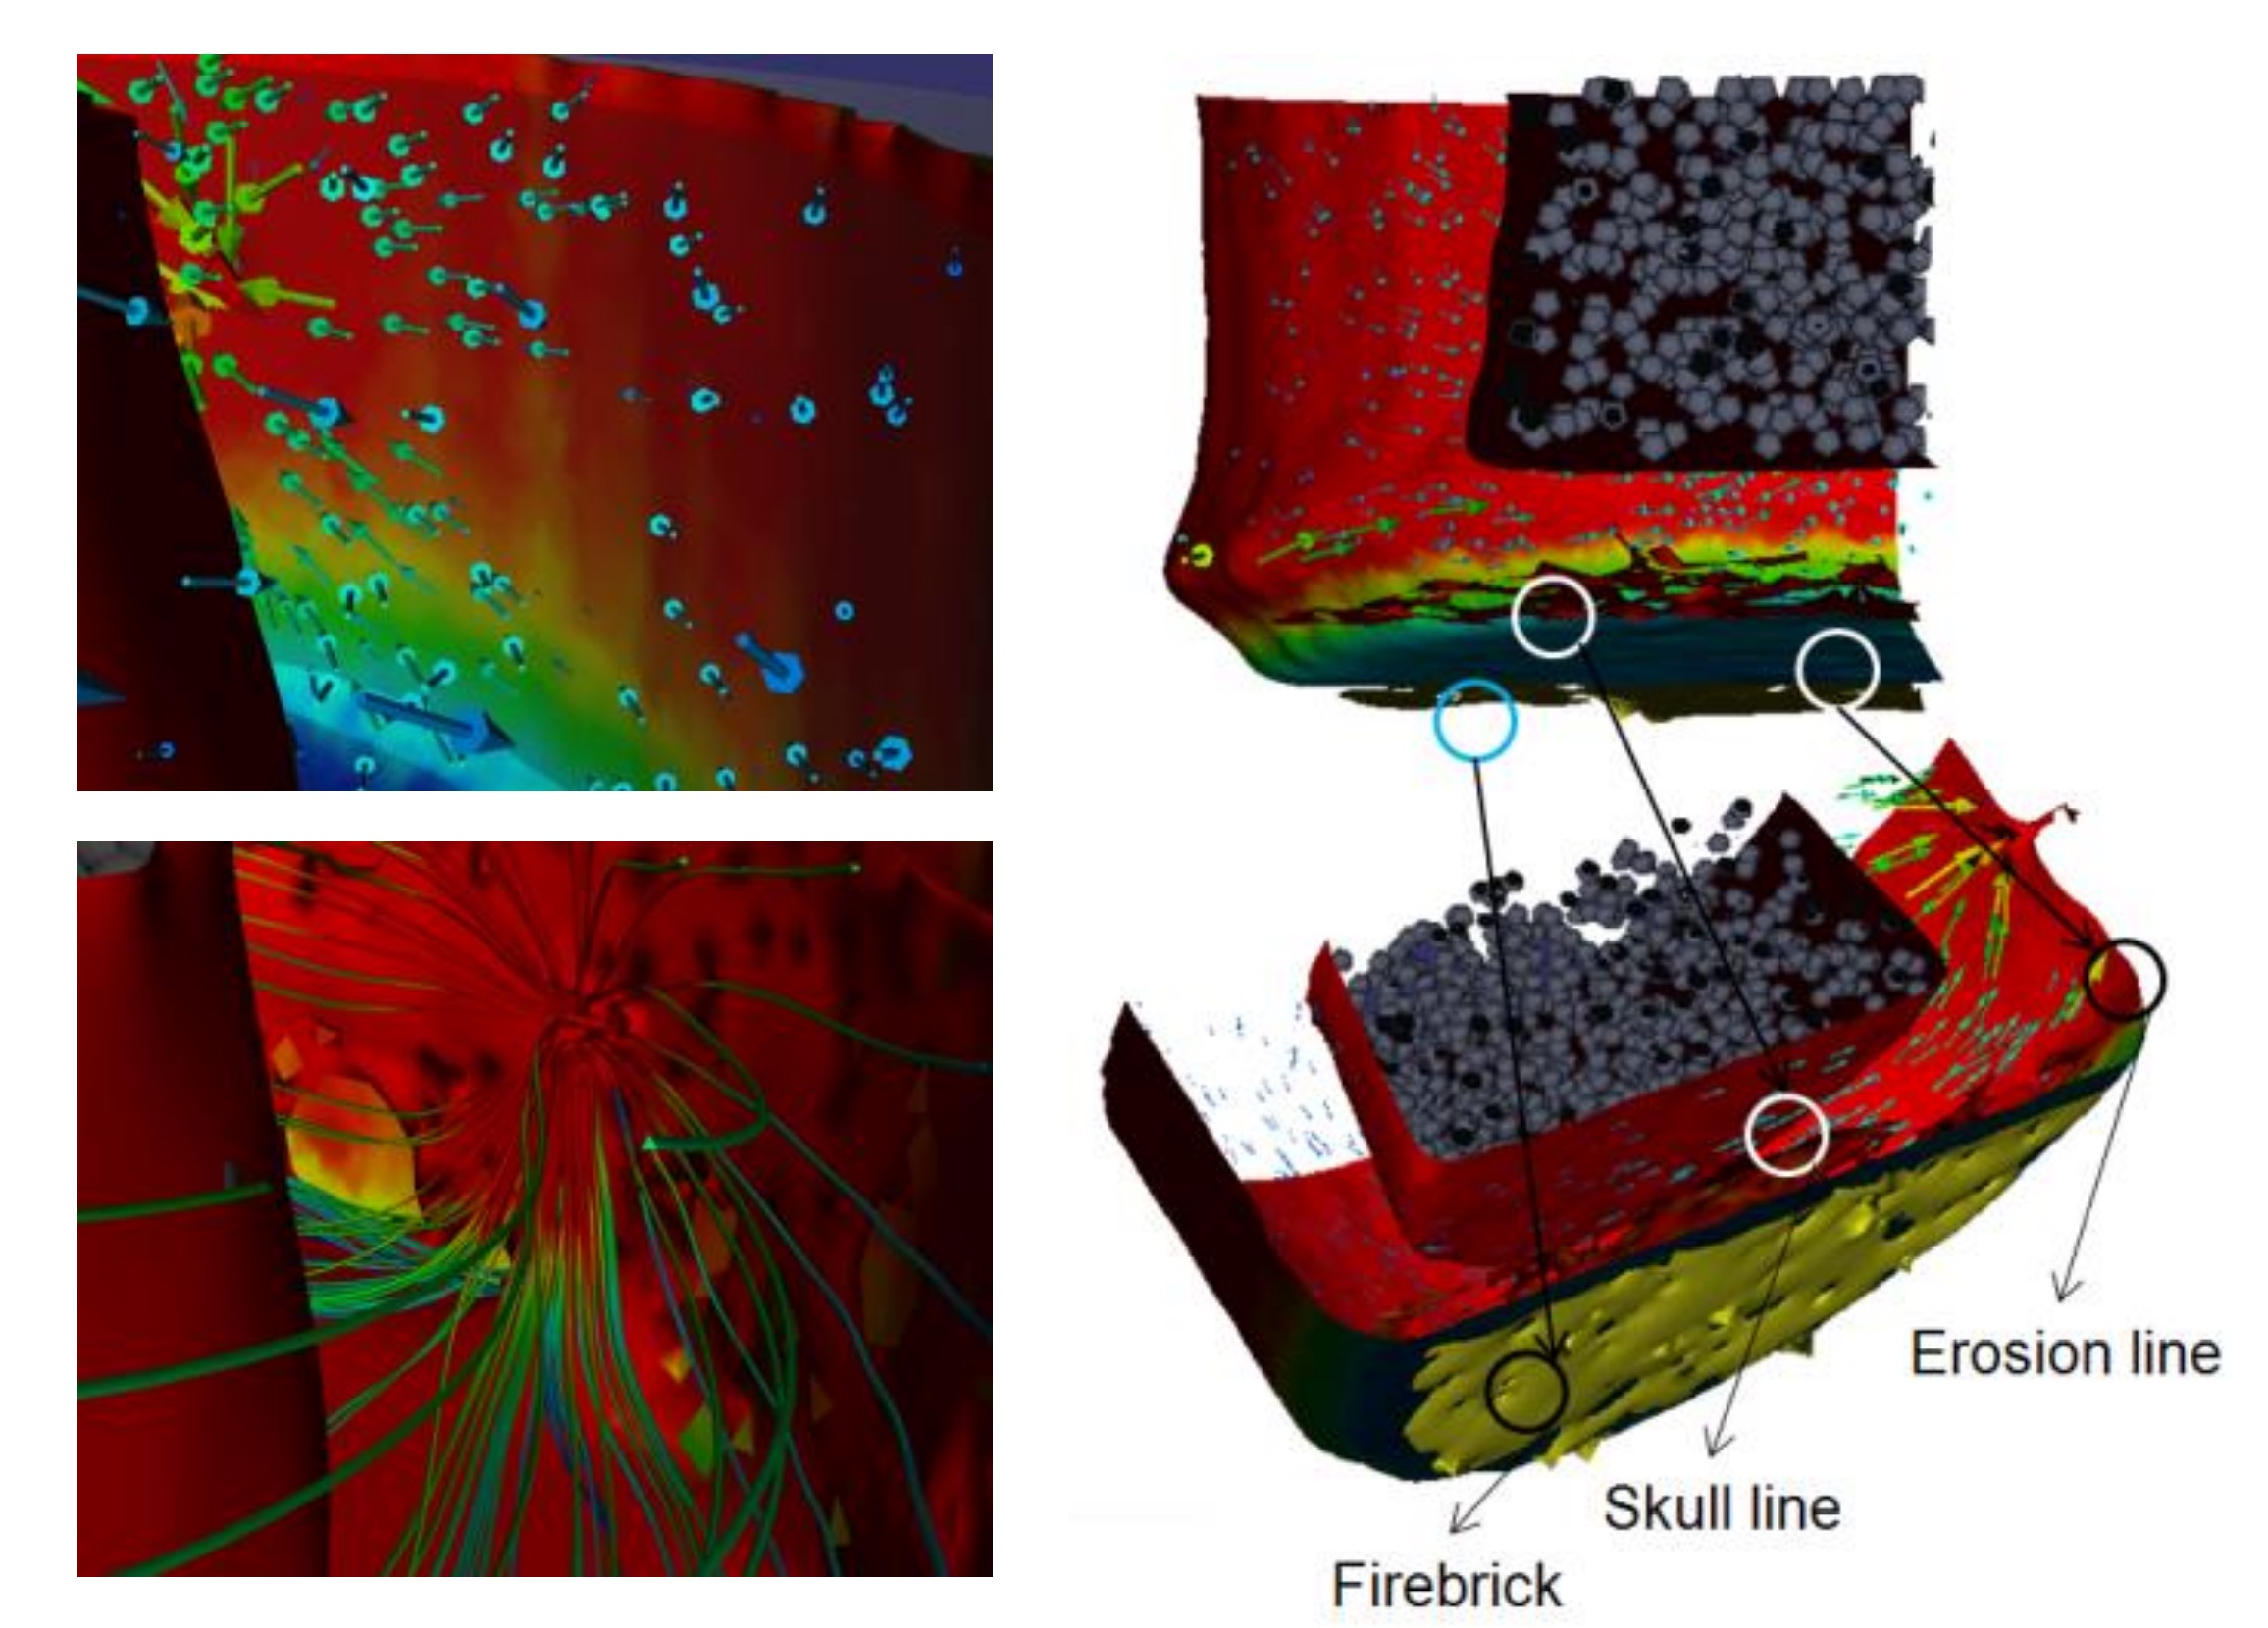
\includegraphics[width=.8\textwidth,angle=0]{figures/blast-furnace-erosion-vr.jpg}
	\caption{3D CFD simulácia vnútra ("srdca") vysokej pece.}
\end{figure}

%Computational fluid dynamics (CFD) has continuously evolved over recent decades and has come to play an important role in the development of modern LD (BOF) steelmaking converters. Flow inside the converter is highly complex and comprises several physical phenomena such as supersonic flow, chemical reactions, heat transfer and the flow of gas bubbles in the liquid melt. For numerical reasons, not all flow processes can be taken into account, but it is possible to describe major effects, show tendencies and gain valuable insight on multi-phase flow processes. The results of these analyses can subsequently be used in the design of new converters. Primetals Technologies is committed to developing an efficient approach to modeling flow and mixing inside the converter during the refining process within a reasonable time. Investigations were carried out on a 110-ton converter in connection with steel bath mixing, which led to the development of a generally applicable method for modeling the flow and quantification of the mixing intensity. It became clear that two kinds of vortices are generated inside the flow, which are of significant importance for mixing and overall flow. On the one hand, vortices are created near the bubble columns at the stirring elements and, on the other hand, much larger vortices are formed that strongly influence the total flow in a molten steel bath. Furthermore, it could be shown that the arrangement and type of bottompurging elements are crucial factors for mixing intensity. An asymmetric alignment of purging elements can result in critical zones inside the converter that are characterized by very low local flow velocities. Primetals Technologies has drawn on its extensive numerical simulation competence to investigate the influence of varying process parameters in order to optimize the overall design of the converter and blowing lance equipment.

%Initial conditions define the starting values for each solution field. They play a vital role in the stability and computing time for steady-state simulations, and are important for getting physically accurate results in transient analyzes. Therefore, it is very important to define appropriate initial conditions for your simulations.
Počiatočné podmienky definujú počiatočné hodnoty pre každé pole riešenia. Zohrávajú dôležitú úlohu v stabilite a výpočtovom čase pre simulácie v ustálenom stave a sú dôležité na získanie fyzikálne presných výsledkov pri analýzach prechodných dejov. Preto je veľmi dôležité definovať vhodné počiatočné podmienky pre vaše simulácie.

Hraničné podmienky určujú, ako systém (napríklad štruktúra alebo tekutina) interaguje s prostredím. Fixácie, zaťaženia, tlaky, prietok alebo rýchlosť tekutiny sú príklady hraničných podmienok.

\subsection{Stlačiteľnosť tekutín}

Kľúčový rozdiel medzi stlačiteľnými a nestlačiteľnými tekutinami je v tom, že stlačiteľné tekutiny sa vyskytujú v reálnom prostredí, zatiaľ čo nestlačiteľné tekutiny, nazývané aj ideálne tekutiny, sú koncepciou vyvinutou na uľahčenie výpočtu.

Kvapaliny, s ktorými sa stretávame v bežnom živote sú do určitej miery stlačiteľné, no 


Stlačiteľnosť tekutiny môžeme definovať ako zmenšenie jej objemu v dôsledku vonkajších tlakov na ňu pôsobiacich. Naopak stlačiteľná tekutina zníži svoj objem v prítomnosti vonkajšieho tlaku. Preto môžeme kvantitatívne meranie stlačiteľnosti vziať ako relatívnu zmenu objemu kvapaliny v reakcii na zmenu tlaku.

Matematicky môžeme stlačiteľnosť $\gamma$ definovať ako

\begin{equation}
	\gamma = \frac{-1}{V} \frac{\partial V}{\partial p}
\end{equation}

kde $V$ je objem tekutiny pred stlačením, $\partial V$ je zmena objemu po sltačení a $\partial p$ je zmena tlaku.

\subsection{Navier-Stokesova rovnica}

Navier-Stokesova (NS) rovnica popisuje prúdenie tekutiny. V praxi má široké využitie, ako napríklad modelovanie minimalizácie odporu vzduchu karosérie áut, návrhu vodných turbín, toku krvi v tele, predpovede počasia a iné. Jej zápis je nasledovný:

\begin{equation}
\frac{\partial \vec{u}}{\partial t} + \vec{u} \cdot \nabla \vec{u} = - \frac{1}{\varrho} \nabla p + \nu \nabla^2 \vec{u} + \vec{g}.
\end{equation}

V praxi sa ňou modeluje hlavne prúdenie nestlačiteľnej (ideálnej) newtonovskej tekutiny, ktorej základná vlastnosť je, že deformácia je priamo úmerná napätiu a jej viskozita je nemenná. Modelovanie stlačiteľnej tekutiny je z hľadiska výpočtového výkonu náročnejšie, čoho dôsledkom je utilizácia vysoko výkonných počítačov a vývoj algoritmov na využitie paralelnej architektúry grafických procesných jednotiek v grafických kartách.

Keďže pri modelovaní systému toku tekutín Navier-Stokesovou rovnicou sa pohybujeme v obore mechaniky tekutín a mechaniky spojitého prostredia (mechanika kontinua), nesmieme zabudnúť na zákon zachovania hmotnosti. Ten popisuje rovnica kontinuity, ktorá v prípade nestlačiteľnej tekutiny nadobúda tvar

\begin{equation}
\frac{\partial \varrho}{\partial t} + \nabla \cdot (\varrho \vec{u}) = 0, 
\end{equation}

kde $\varrho$  je hustota, $t$ je čas, $\nabla \cdot$ je divergencia a $\vec{u}$ je vektorové pole rýchlosti prúdenia.

Pri nestlačiteľnej tekutine zostáva hustota pozdĺž toku v priebehu času konštantná (teda nemenná)

\begin{equation}
\frac{\partial \varrho}{\partial t} = 0, 
\end{equation}

z čoho vyplýva, že divergencia vektorového poľa rýchlosti prúdenia je nulová

\begin{equation}
\nabla \cdot \vec{u} = 0.
\end{equation}


%X-moment:
%
%\begin{equation}
%\frac{\partial (\varrho u)}{\partial t} + \frac{\partial (\varrho u^2)}{\partial x} + \frac{\partial (\varrho uv)}{\partial y} + \frac{\partial (\varrho uw)}{\partial z} = - \frac{\partial p}{\partial x} + \frac{1}{Re} \left[\frac{\partial \tau_{xx}}{\partial x} + \frac{\partial \tau_{xy}}{\partial y} + \frac{\partial \tau_{xz}}{\partial z}\right]
%\end{equation}
%
%Y-moment:
%
%\begin{equation}
%\frac{\partial  (\varrho v)}{\partial t} + \frac{\partial (\varrho uv)}{\partial x} + \frac{\partial (\varrho v^2)}{\partial y} + \frac{\partial (\varrho vw)}{\partial z} = - \frac{\partial p}{\partial x} + \frac{1}{Re} \left[\frac{\partial \tau_{yx}}{\partial x} + \frac{\partial \tau_{yy}}{\partial y} + \frac{\partial \tau_{yz}}{\partial z}\right]
%\end{equation}
%
%Z-moment:
%
%\begin{equation}
%\frac{\partial  (\varrho w)}{\partial t} + \frac{\partial (\varrho uw)}{\partial x} + \frac{\partial (\varrho vw)}{\partial y} + \frac{\partial (\varrho w^2)}{\partial z} = - \frac{\partial p}{\partial x} + \frac{1}{Re} \left[\frac{\partial \tau_{zx}}{\partial x} + \frac{\partial \tau_{zy}}{\partial y} + \frac{\partial \tau_{zz}}{\partial z}\right]
%\end{equation}

Vo všeobecnosti sú NS rovnice v realite nelineárne parciálne diferenciálne rovnice. Tieto nelinearity sú zodpovedné za turbulencie, ktoré vznikajú pri prúdení tekutín a ktoré tieto rovnice modelujú. Dôvodom vzniku nelinearít je konvekčné zrýchlenie, teda zrýchlenie šírenia tepla prúdením. 

Turbulencia je chaotické správanie sa mnohých tekutín. Riešenie NS rovníc pre turbulentné prúdenie tekutiny je extrémne obtiažne, keďže pre dosiahnutie stabilného riešenia je potrebná veľmi detailná sieť. 

Aj napriek praktickému využitiu, zatiaľ neexistuje dôkaz o tom, či riešenia NSR vždy existujú v troch dimenziách, a ak áno, tak či sú na celom intervale nekonečne diferencovateľná. Na tento problém Clayov inštitút vypísal odmenu 1 milión dolárov.

\subsection{Metóda lattice Boltzmann}

Metóda lattice Boltzmann je relatívne nová metóda v oblasti CFD analýzy.


\citep{delbosc2015}


Boltzmannova rovnica je základná evolučná rovnica pre kontinuum, popísanej v šesť-dimenzionálnom fázovom priestore. Rovnica popisuje vývoj distribučnej funkcie v čase. Tá sa môže meniť v dôsledku vzájomných kolízií častíc, ktoré pri nárazoch menia svoju hybnosť a energiu, a to v dôsledku vlastného pohybu častíc alebo vplyvom externých síl \citep{HEIDLER2011thesis}.

LBM vychádza z z 

%Over the past few decades, tremendous progress has been made in the development of particle-based discrete simulation methods versus the conventional continuum-based methods. In particular, the lattice Boltzmann (LB) method has evolved from a theoretical novelty to a ubiquitous, versatile and powerful computational methodology for both fundamental research and engineering applications. It is a kinetic-based mesoscopic approach that bridges the microscales and macroscales, which offers distinctive advantages in simulation fidelity and computational efficiency. Applications of the LB method are now found in a wide range of disciplines including physics, chemistry, materials, biomedicine and various branches of engineering.

V posledných niekoľkých desaťročiach sa dosiahol obrovský pokrok vo vývoji diskrétnych simulačných metód založených na časticiach v porovnaní s konvenčnými metódami založenými na kontinue. Najmä sa metóda mriežky Boltzmann (LB) vyvinula z teoretickej novosti na všadeprítomnú, všestrannú a výkonnú výpočtovú metodológiu pre základné výskumné aj inžinierske aplikácie. Jedná sa o kineticky založený mezoskopický prístup, ktorý premosťuje mikroskopické a makroskopické mierky, čo ponúka výrazné výhody pri vernosti simulácie a výpočtovej účinnosti. Aplikácie metódy LB sa v súčasnosti nachádzajú v širokej škále odborov vrátane fyziky, chémie, materiálov, biomedicíny a rôznych odborov strojárstva.

\begin{figure}[!ht]
	\centering
	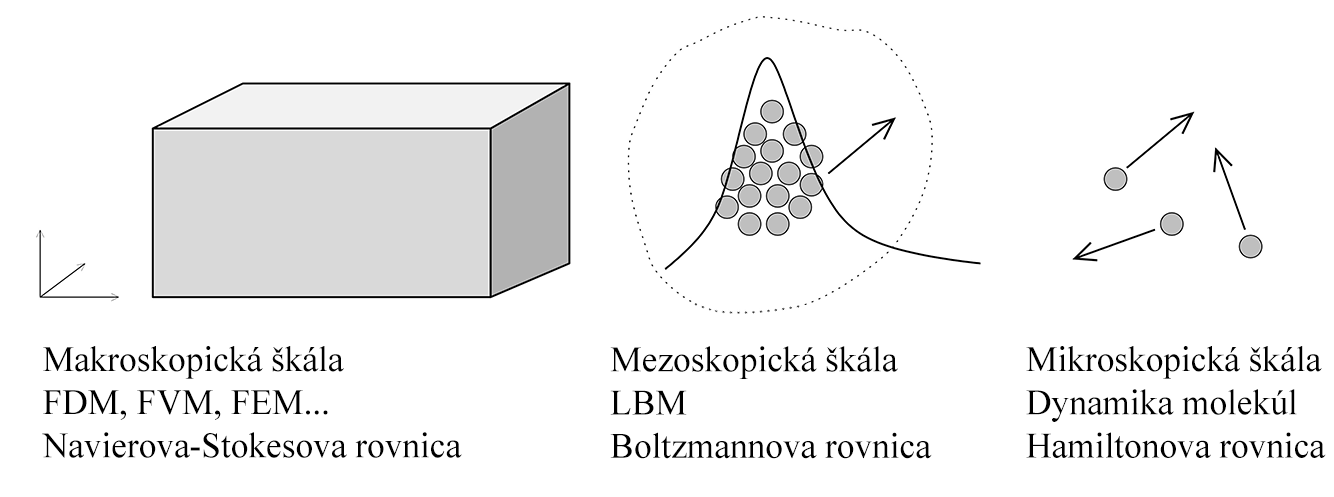
\includegraphics[width=1\textwidth,angle=0]{figures/different-scales.png}
	\caption{Techniky simulácie v rôznych škálach \citep{Mele2013}.}
\end{figure}

%The particles jump from one lattice node to the next, according to their (discrete) velocity. This is the propagation phase
Častice skočia z jedného mriežkového uzla do nasledujúceho podľa svojej (diskrétnej) rýchlosti. Toto je propagačná fáza

%Then, the particles collide and get a new velocity. This is the collision phase
Potom sa častice zrazia a získajú novú rýchlosť. Toto je fáza kolízie

%Rules governing the collisions are designed such that the time-average motion satisfies mass and momentum conservation
Pravidlá upravujúce zrážky sú navrhnuté tak, aby priemerný čas vyhovoval zachovaniu hmotnosti a hybnosti

\begin{figure}[!ht]
	\centering
	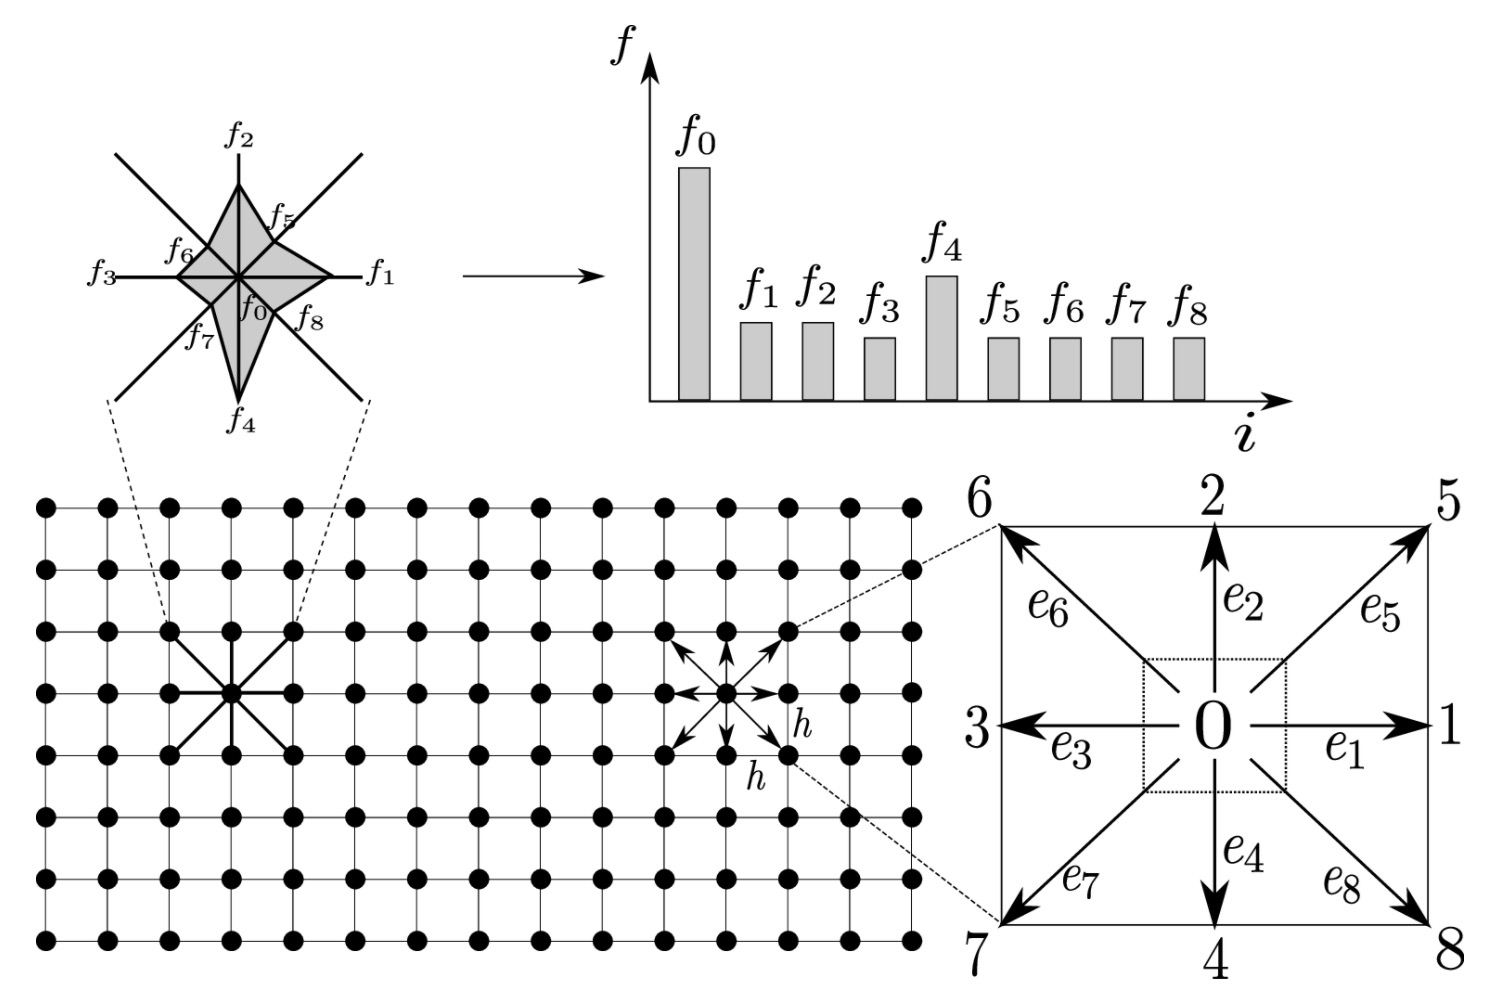
\includegraphics[width=.7\textwidth,angle=0]{figures/lbm-grid.jpg}
	\caption{Mriežková štruktúra LBM \citep{Soga2020}.}
\end{figure}

Pri LBM sa (ako aj pri iných numerických metódach) môže objaviť numerická nestabilita. Zatiaľ pre túto metódu nie sú presne dané podmienky stability, ale z doterajších praktických výpočtov vzišlo niekoľko podmienok, pri ktorých držaní sa je možné dosiahnuť akceptovateľnú stabilitu:

\begin{enumerate}
	\item{Kinetická viskozita by mala byť kladná.}
	\item{Výsledná makroskopická rýchlosť prúdenia}
\end{enumerate}


\subsection{Modelovanie turbulencie}

LES (Large Eddy Simulation) je matematický model turbulencie pôvodne navrhnutý Josephom Smagorinskym


$K-\epsilon$ je matematický model turbulencie

\subsection{DNS}

Direct Numerical Simulation

\section{Programy pre CFD simulácie}

\subsection{Matlab}
Matlab obsahuje niekoľko toolboxov pre CFD analýzu. 

\subsection{Ansys Fluid}

Ansys Fluid

\subsection{SimScale}

Platforma SimScale ponúka v rámci čiastkových produktov mnohé funkcionality ako ostatné simulačné programy, no táto firma stavila na využitie cloudových technológií. Práca s programom prebieha cez webové rozhranie, kde užívateľ nastavuje a spúšťa simulácie a taktiež sa priamo vo webovom prehliadači zobrazuje 2D alebo 3D vizualizácia simulovaného modelu. Výpočty prebiehajú na serveroch prevádzkovaných alebo prenajímaných firmou SimScale, ktoré využívajú možnosti masívnej paralelizácie grafických kariet


\begin{figure}[!ht]
	\centering
	\subfloat[Simulácia toku vetra okolo modelu niekoľkých výškových budov so zložitou geometriou.]{{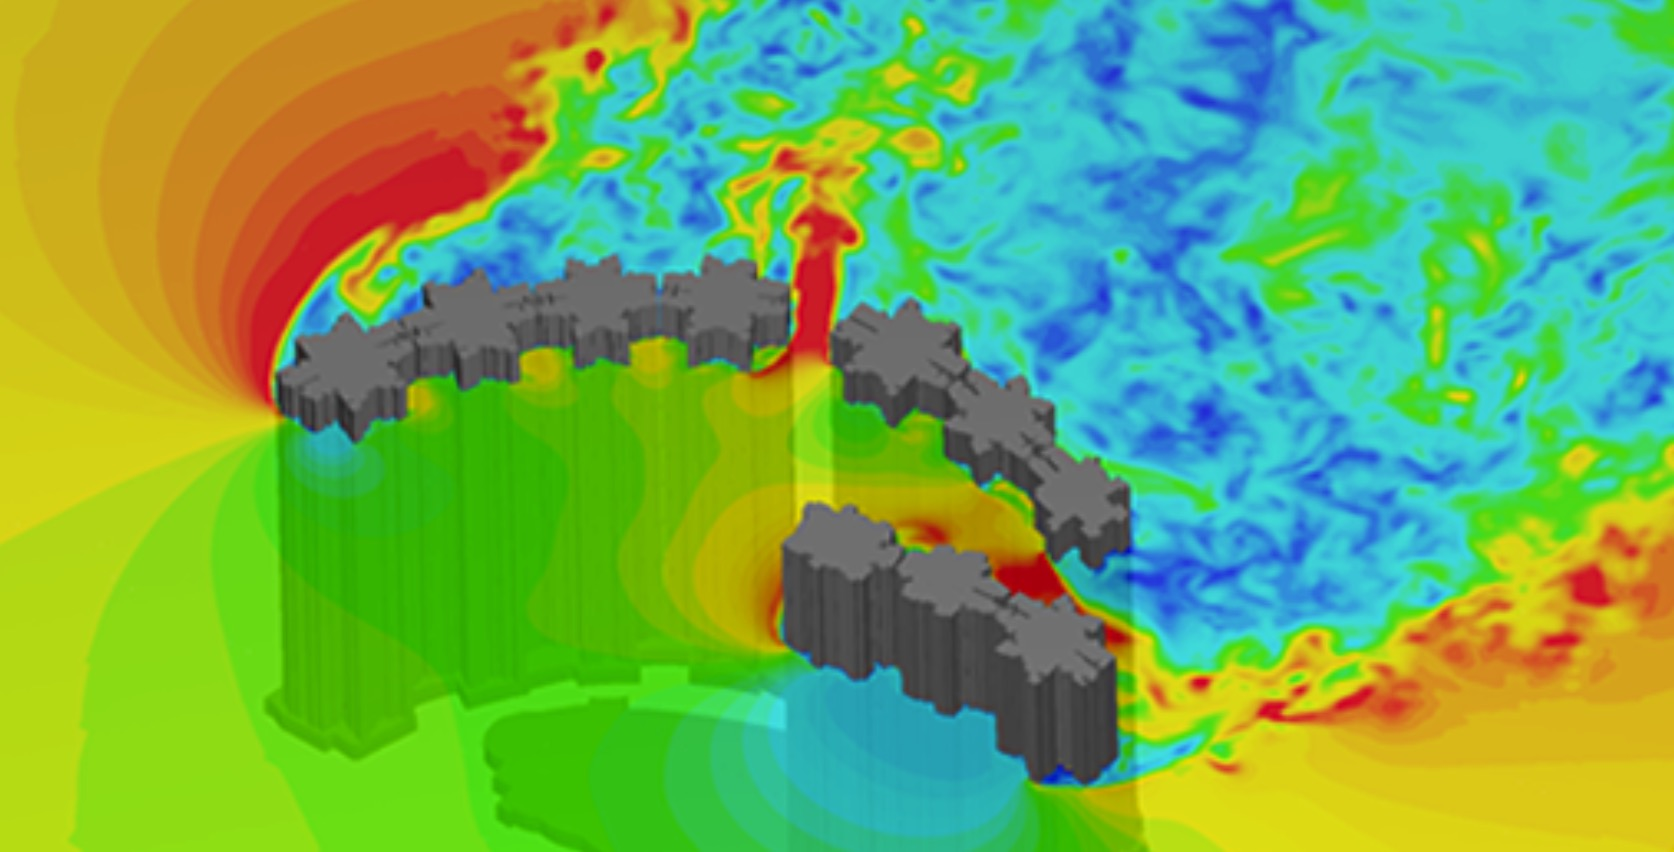
\includegraphics[width=7.1cm]{figures/simscale-cfd.jpg} }}%
	\qquad
	\subfloat[CFD simulácia viacfázovej tekutiny.]{{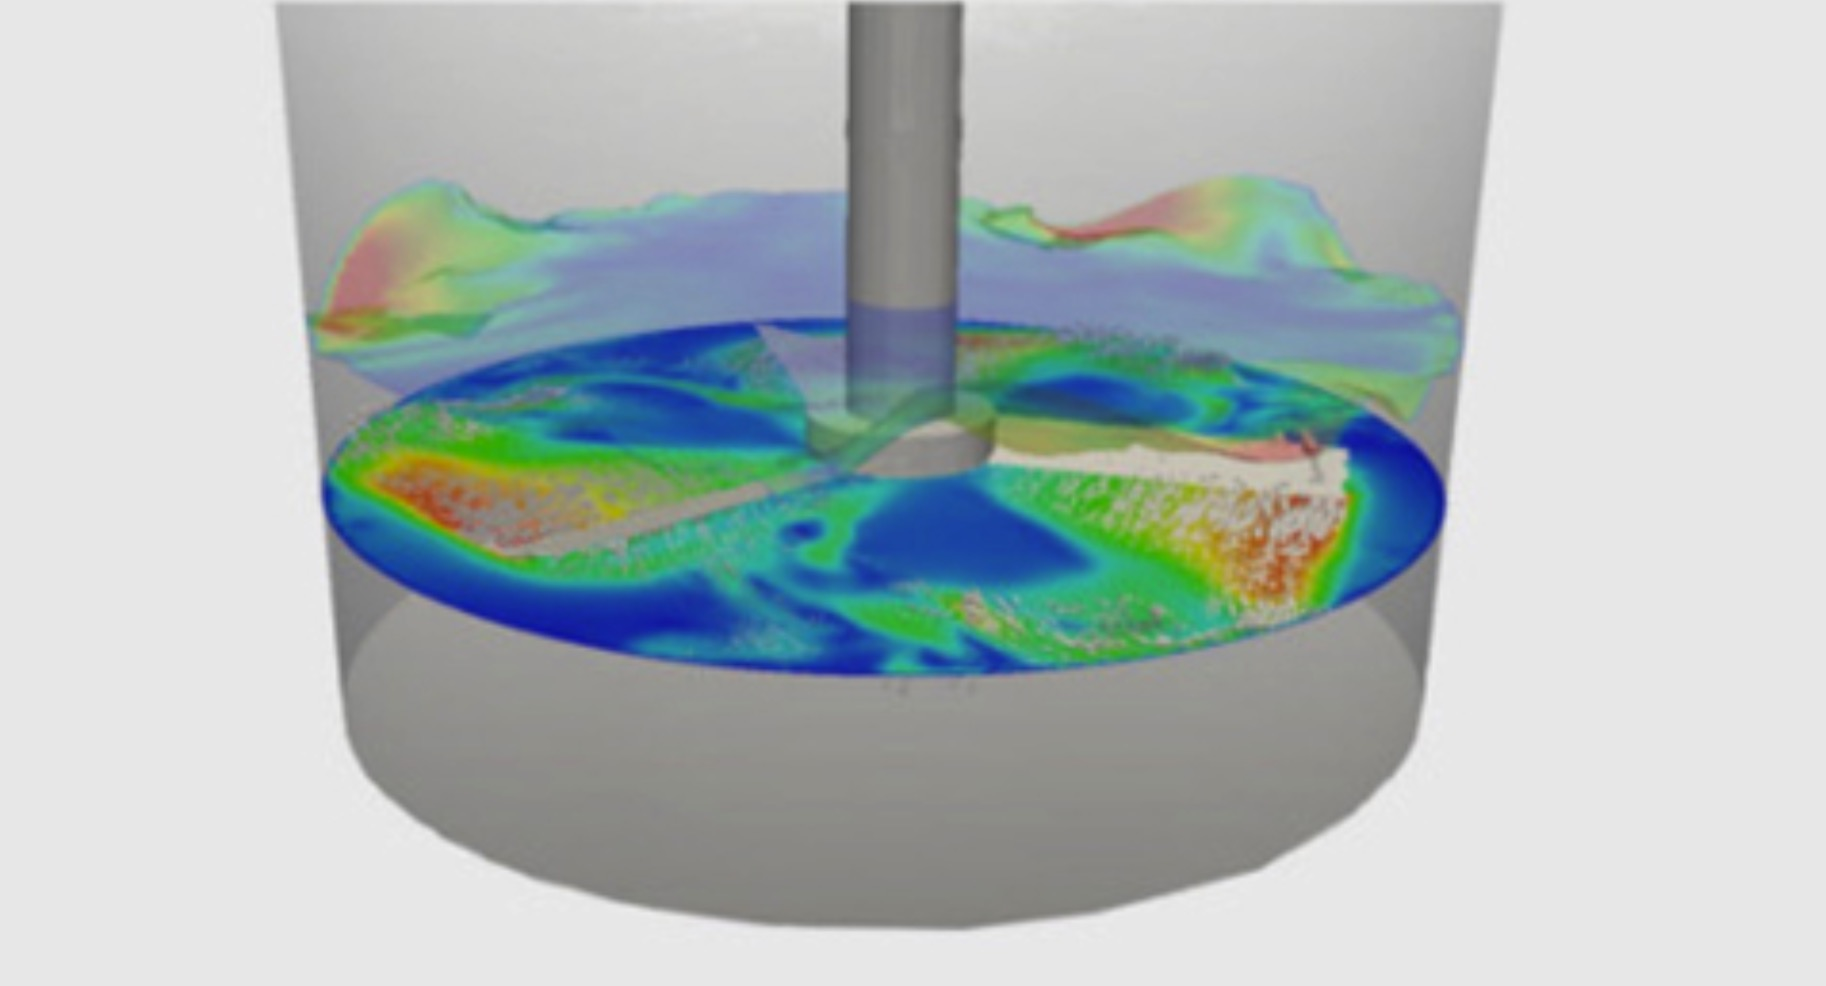
\includegraphics[width=6.7cm]{figures/simscale-multiphase.jpg} }}
	\caption{Vizualizácie CFD simulácií v prostredí SimScale.}
\end{figure}

\subsection{OpenFOAM}

%is a toolbox for solving complex Computational Fluid Dynamics problems. It contains a wide range of physical models (including turbulence, wall treatment, thermodynamics, and mass transport), numerical methods and tools for pre- and post-processing.

OpenFOAM je súbor nástrojov s voľne prístupným zdrojovým kódom na riešenie zložitých problémov s výpočtovou dynamikou tekutín. Obsahuje širokú škálu fyzikálnych modelov (vrátane turbulencie, úprav stien hraničných podmienok - geometrie, termodynamiky a hromadnej dopravy), numerických metód a nástrojov na predbežné a následné spracovanie.

\subsection{OpenLB}

OpenLB je balík C++ modulov pre implementáciu lattice Boltzmann simulácií určený predovšetkým ako programová podpora pre výskumníkov a technikov, ktorí simulujú toky tekutín pomocou LBM. Podporuje komplexné dátové štruktúry, pomocou ktorých je možné simulovať zložité geometrie. Diskretizovať geometrie (meshing alebo voxelizácia) z dopredu pripravených 3D modelov a nastaviť okrajové podmienky je možné automaticky - automatickým predspracovaním (aj komplexného) 3D modelu. Paralelizácia v implementovaných algoritmoch je riešená využitím knižnice OpenMP, z čoho môžu benefitovať výkonné multiprocesorové viacjadrové počítače (v architektúrach využívajúcich zdieľanú pamäť). Pri distribuovaných počítačových systémoch, na ktorých by sme chceli simulovať modely na báze LBM pomocou OpenLB majú paralelné algoritmy v tomto balíku implementované rozhranie na posielanie a prijímanie správ medzi jednotlivými procesmi (MPI - Message-Passing Interface

\section{Záver}

Simulácie sú v súčasnosti už neoddeliteľnou súčasťou počítačom podporovaného inžinierstva ako aj vedeckého skúmania fyzikálnych javov. Výsledkom simulácie je približné, no dostatočne presné riešenie modelovanej úlohy. Modelovanie na základe matematických metód prešlo dekádami vývoja a vylepšovanie metód pokračuje naďalej.  

%
%%
\Urlmuskip=0mu plus 1mu\relax
\bibliographystyle{spbasic}
\bibliography{refs/control,refs/mathematics,refs/modeling,refs/cfd,refs/lbm,refs/gpu,refs/interaction,refs/interfaces,refs/hci,refs/design,refs/ml,refs/visualization,refs/programming,refs/simulation,refs/ar,refs/vr,refs/online}

%

\end{document}
%%